\documentclass[a4paper,10pt]{article}
\usepackage[utf8]{inputenc}
\usepackage{amsmath,amssymb}
\usepackage{listings}
\usepackage{graphicx}

%opening
\title{Aufgabe 07}
\author{Can Nayci, Leonhard Rattmann, Emil Sharaf}
\date{09.12.2023}
\begin{document}

\maketitle

\section{Circle}
\begin{align*}
 N &: \text{Anzahl der Elemente des Arrays} \\
 nprocs &: \text{Anzahl der Prozesse} \\
 start_p &: \text{erstes Element für Prozess } p\\
 end_p &: \text{letztes Element für Prozess } p\\
 start_0 &= 1 \\
 end_p &= p \cdot (int) \frac{N}{nprocs} + a\\
 a &=
 \begin{cases}
    \text{wenn }((N \bmod nprocs) < p) : 0\\
    \text{sonst} : 1\\
 \end{cases}\\
 start_p &= end_{p-1}\\
\end{align*}\\
für $N = 13, nprocs = 5$:
\begin{tabular}{c | c}
 Prozess & Array-Elemente \\
 \hline
 0 & $0,1,2$\\
 1 & $3,4,5$\\
 2 & $6,7,8$\\
 3 & $9,10$\\
 4 & $11,12$\\
\end{tabular}


%%
\section{Visualisierung}
\begin{itemize}
    \item[1] \textbf{Grafische Darstellung der Kommunikation:}\\\\
    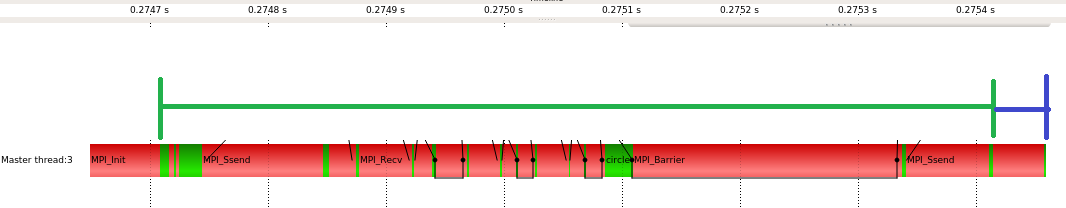
\includegraphics[width=14cm]{GrafikKommunikation.png}
    \item[2] \textbf{Communication Matrix View:}\\\\
    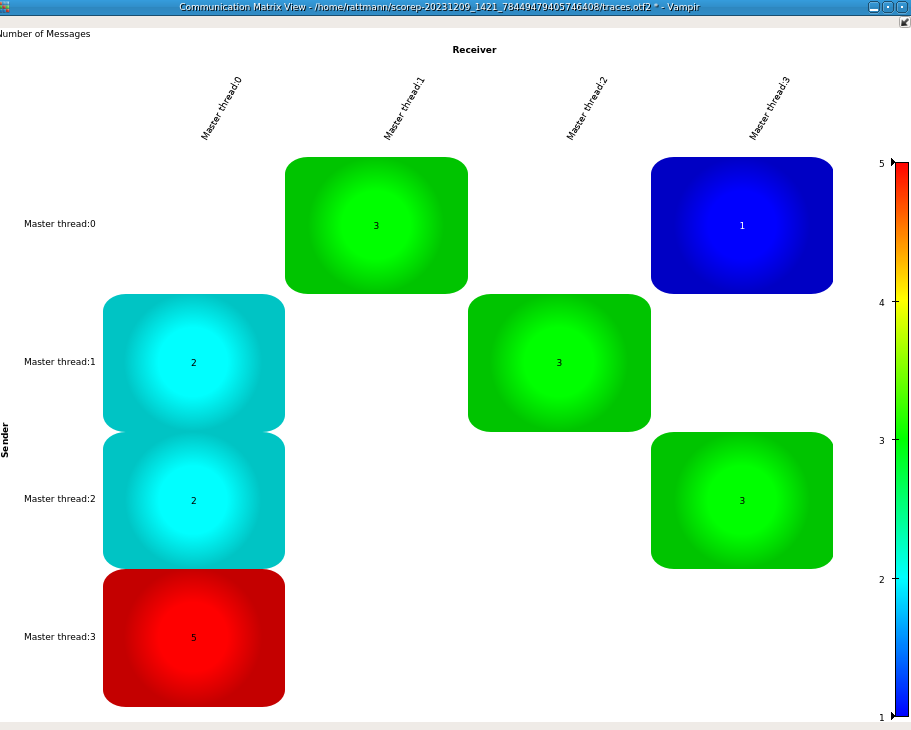
\includegraphics[width=14cm]{CommunicationMatrixView1.png}\\
    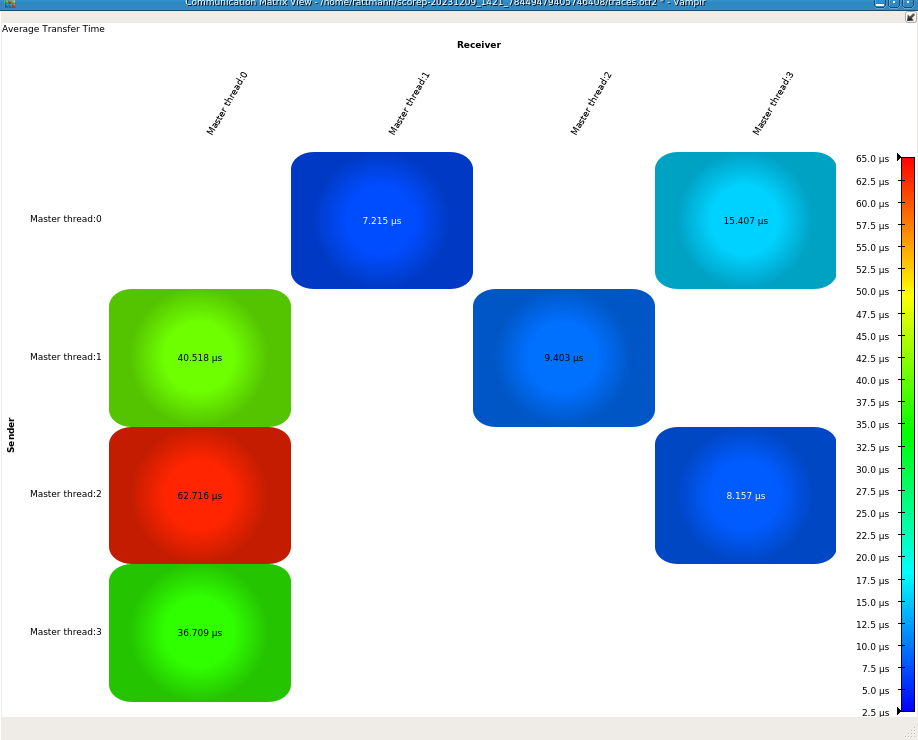
\includegraphics[width=14cm]{CommunicationMatrixView2.png}\\
    \item[3]\textbf{Programmphasen:}\\\\
    Die Phase bis $0,2747$ s stellt die Initialisierung dar. Die Iterationen werden in den nachfolgenden Screenshots als "grüne Phase" und das Beenden als "blaue Phase" dargestellt:\\\\
    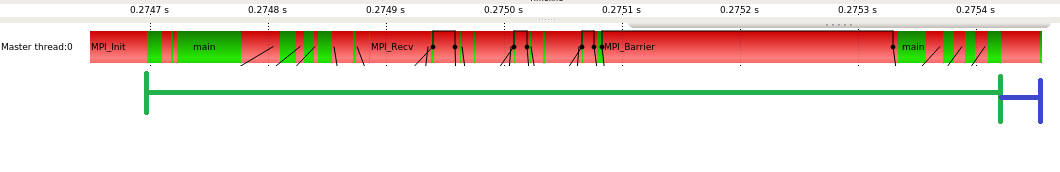
\includegraphics[width=14cm]{Init_1.png}\\
    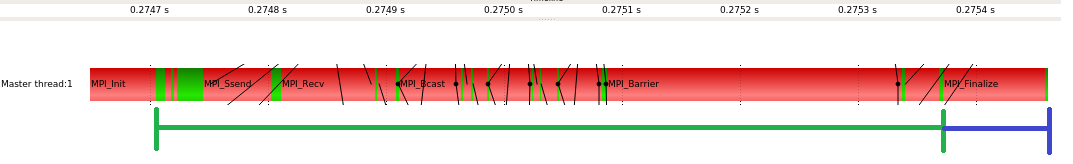
\includegraphics[width=14cm]{Init_2.png}\\
    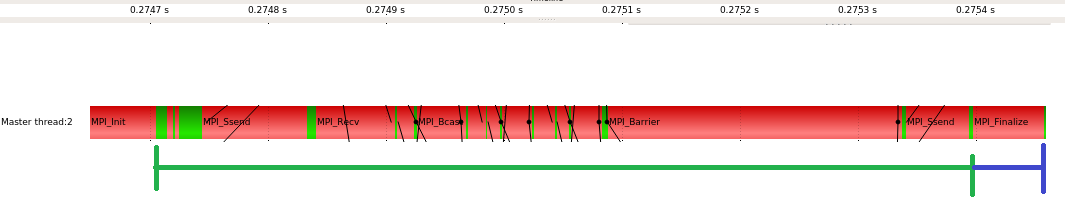
\includegraphics[width=14cm]{Init_3.png}\\
    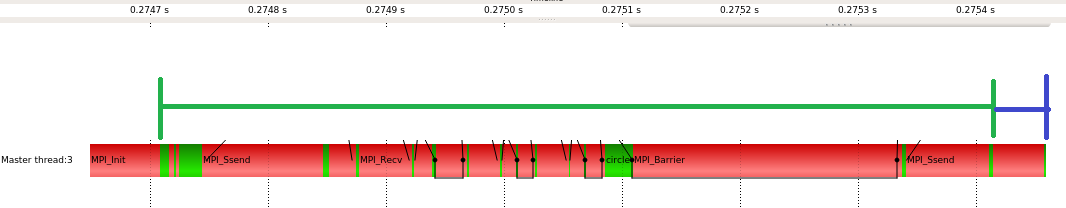
\includegraphics[width=14cm]{Init_4.png}\\
    \item[4] \textbf{MPI-Init-Phase:}\\\\
    Die MPI-Init-Phase dauerte $\thicksim 1,098$ s und nimmt somit ungefähr 99,7\% der Programmlaufzeit in Anspruch:\\\\
    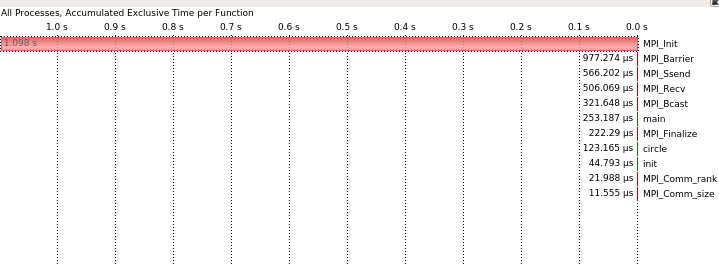
\includegraphics[width=14cm]{MPI_Init.png}
\end{itemize}
\newpage
\section{Prallelisierung mit MPI}

\begin{lstlisting}[language=C]
 int n = Anzahl der Reihen;
 int nprocs = Prozessanzahl;
 n = (getInterlines() * 8) + 9 - 1;
 int startIndex, endIndex;

 nur Prozess 0:
 {
    int s_startIndex, s_endIndex;
    int lpp, lpp_rest;

    lpp = (int) (n - 1) / nprocs;
    lpp_rest = (n - 1) % nprocs;

    startIndex = 1 (0er-Reihe wird ignoriert);
    endIndex = lpp + (lpp_rest < 0)? 1 : 0);
    lpp_rest--;

    s_startIndex = endIndex;
    s_endIndex = 0;
     fuer alle nprocs exkl. 0:
    {
        MPI_Ssend(*s_startIndex an Prozess i);
        s_endIndex = startIndex + lpp;
        if (lpp_rest < 0)
        {
            endIndex++;
            lpp_rest--;
        }
        MPI_Ssend(*s_endIndex an Prozess i);
        s_startIndex = s_endIndex;
        // => startIndex ist inklusive, endIndex exklusive.
    }
 }

 alle anderen Prozesse:
 {
    MPI_Recv(*startIndex);
    MPI_Recv(*endIndex);
 }

\end{lstlisting}

z.B. 64 Interlines, 4 Prozesse:
\begin{align*}
  & &n = 64 * 8 + 9 - 1 = 520\\
  & &lpt = \frac{519}{4} = 129 \\
  & &lpt\_rest = 3 \\
 &\text{für Prozess 0: }
 &startIndex = 1 \\
 & &endIndex = 130 + 1\\
 &\text{für Prozess 3: }
 &startIndex = 262\\
 & &endIndex = 391 + 1\\
 &\text{für Prozess m:  }
 &startIndex = 1 + m \cdot lpt + lpt\_rest \\
  & &\text{nicht $(m - 1)$, weil Prozesse ab 0 nummeriert sind}\\
 & &endIndex = 521\\
\end{align*}
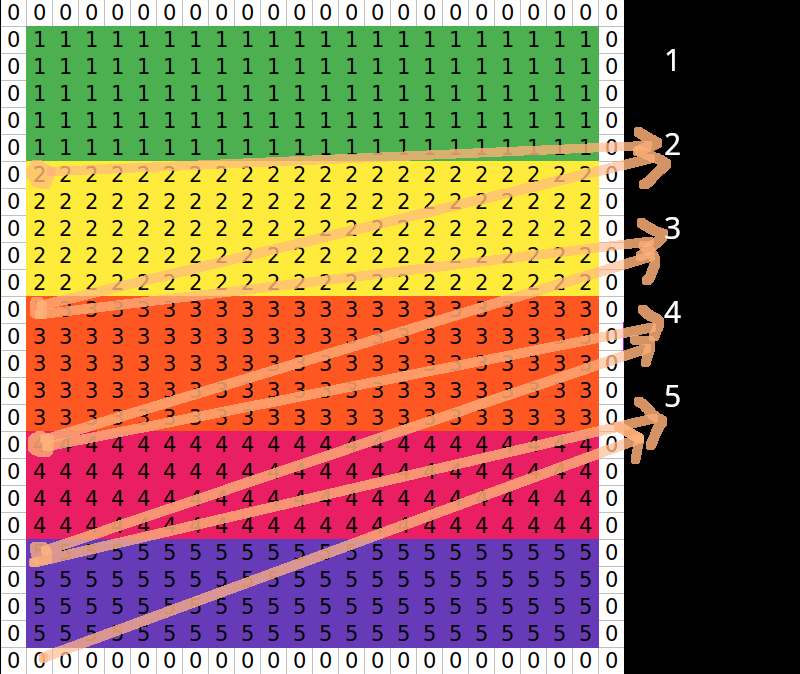
\includegraphics[width=8cm]{Untitled.png}
\subsection*{Kommunikation}
1. Alle Prozesse außer 0 (bzw. 1) brauchen ihre Start- und endIndizes.
2. Jeder Prozess braucht in jeder Iteration den oben und unten benachbarten Teil der Matrix.


\end{document}
